\documentclass[12pt, letterpaper]{report}

% Set 1 inch margins
\usepackage[margin=1in]{geometry}
\usepackage{amsmath}
\usepackage[colorlinks=true, linkcolor=black, urlcolor=blue, citecolor=black]{hyperref}
\usepackage{tikz}
\usetikzlibrary{positioning, decorations.pathreplacing, decorations.pathmorphing, patterns, shapes, decorations.text}
\definecolor{gold}{RGB}{207, 181, 59}
\usepackage{librecaslon}
\usepackage[T1]{fontenc}

% Use ragged right justification (left-align text)
\usepackage[document]{ragged2e}

% Set bold chapter and section headings
\usepackage{titlesec}
\titleformat{\chapter}[hang]{\normalfont\Large}{\thechapter}{2pc}{}
\titleformat{\section}[hang]{\normalfont}{\thesection}{1pc}{}

% For list of figures and tables
\usepackage{tocloft}
\setlength{\cftfigindent}{0pt}
\setlength{\cfttabindent}{0pt}

% TOC formatting
%\renewcommand{\cftchapleader}{\cftdotfill{\cftdotsep}}
\renewcommand{\cftchapfont}{\normalfont}  % Remove bold from chapter entries
\renewcommand{\cftsecfont}{\normalfont}   % Remove bold from section entries
\renewcommand{\cftchappagefont}{\normalfont} 
\renewcommand{\cftsecpagefont}{\normalfont} 

% For bibliography
\usepackage{cite}
\renewcommand{\bibname}{References}  % Change "Bibliography" to "References"

% Additional packages for figures and tables
\usepackage{graphicx}
\usepackage{caption}
\usepackage{subcaption}
\usepackage{booktabs} % For table formatting

% Paragraph indentation and hyphenation settings
\setlength{\parskip}{1em}
\hyphenpenalty=500          % Reduces the amount of hyphenation
\exhyphenpenalty=1000       % Prevents hyphenation across lines


% Document parameters
\def\title{The title of the dissertation using sentence case: First word of subtitle capitalized}
\def\student{Student P. Name}

% Document begins
\begin{document}
\pagenumbering{roman}

% Title Page
\thispagestyle{empty}
\rule{0pt}{0pt}{\centering
\vfill
{\LARGE\title\par}
\vfill
\rule{0pt}{1in}\\
{\Large\student}\\
\rule{0pt}{1in}\\
\vfill
{\large A dissertation for the\\
Doctor of Philosophy degree\\
presented to the faculty of the\\
School of Data Science\\
University of Virginia\\
on 23 April 2024\\
}}
\vfill
\rule{0pt}{0pt}
\newpage
% Committee page
\thispagestyle{empty}
\addcontentsline{toc}{chapter}{Committee}
\rule{0in}{1in}
\begin{center}
{\large 
\begin{tabular}{l}
Dissertation committee\\
    \ \\
John Conway, Advisor\\
Isaac Newton, Chair\\
Florence Nightengale\\
Katherine Johnson\\
Kermit T. Frog
\end{tabular}
}
\end{center}
\newpage
\chapter*{Abstract}
\addcontentsline{toc}{chapter}{Abstract}

\begin{center}
{\large\title\par}

{\student}
\end{center}
The following abstract is from the dissertation of Natalie Kupperman, PhD.  Athlete monitoring is the practice of collecting data in athletics to quantify load, both physical and mental, with the goal to reduce fatigue, optimize performance and mitigate injury risk. The influx in technology over past 15 years has given practitioners the ability to quantify these measures at an increased frequency. However, the subsequent research that followed has found limited associations between these measures and injury risk. There are many possible reasons for this paucity, one of which is the methods used to investigate these data. The purpose of this dissertation was to use three different methodological techniques to both introduce novel analysis to the field and also highlight the need for within-person design in athlete monitoring.

The purpose of manuscript 1 was to evaluate differences in external workload trends of athletes who sustained an overuse injury during sport. We did this using a case series format to evaluate differences in on-court volume, as measured by whole-body accelerometry, of three court-sport athletes and three position-matched healthy control athletes. Across sports, teams, and sexes, we found differences in accelerometer data between injured athletes and healthy matched controls in the 8 weeks leading up to the injury. The injured volleyball athlete had greater accumulated playerload per min (PL/min), jumps per minute and duration compared to the healthy athlete across the 8 weeks. For basketball, both injured athletes had greater PL/min compared to their controls, however, jumps per min were less than the healthy athletes over the 8 weeks.

The purpose of manuscript 2 was to a apply longitudinal structural equation modeling framework to athlete monitoring data with the goal of better understanding between- and within-person differences. Longitudinal athlete sport participation status and self-reported wellness were collected from 16 volleyball athletes and aggregated into weekly observations over 5 weeks. Three models – univariate latent curve model (LCM), LCM with structured residuals (SR), and LCM-SR with time varying covariates – are described. Then using simulated data based off the 16 athletes, results for each model are reported and substantively interpreted. The final model shows statistically significant effects of wellness on both the same and subsequent week athlete availability.

The purpose of manuscript 3 was to first introduce a research design using machine learning (ML) and explanatory model that is new the field of athlete monitoring and the use a case study in collegiate basketball to demonstrate the proposed research design. The research design contained 3 steps. First, data was processed using an ML algorithm designed for feature selection. Then based on the important features defined by the ML algorithm and researcher input, variables are selected, and a testable hypothesis is generated. The hypothesis was then tested using an explanatory model. The external load and readiness datasets performed best with ordinal forests, whereas the athlete self-report measures data did best with an support vector machine. Readiness had the best performance with MSE = 0.89. For the explanatory model, only the physical performance capability (PPC) model was statistically significant. This model found the odds having above average soreness decrease by 57\% for every point increase in PPC (OR=0.57, 95\% CI 0.32 to 0.97, p<0.05).

In undertaking these studies, the complexities of modeling injury were demonstrated. There is still much to be explored; however, by attempting new ways of analyzing athlete monitoring, we were able to highlight the need for continued forward thinking in methodologies, both at the level of analysis and the analytical tools employed. 

\newpage
\chapter*{Acknowledgements}
\addcontentsline{toc}{chapter}{Acknowledgements}
From the dissertation of Phil Bourne.  I am exceedingly grateful to Dr. M. R. Taylor for his supervision during my candidature for this degree. Special thanks must also go to Mr. J. Drennan and Ms M. J. McCall who were a continuous source of inspiration, and who will long be remembered. Thanks also to Drs. N. Latavalya and E. Summerville, Mr. J. Mohyla and Professor D. J.M. Bevan who provided useful comments and Mr. J. A. Westphalen who was always helpful in running XRAY-76 on the CDC7600 at The South Australian Institute of Technology.

People external to The Flinders University of South Australia who should be acknowedged are Drs. A. H. White and C. L. Raston for the 4-circle diffractometer data sets collected at The University of Western Australia and Prof. G. M. Sheldrick for his personal introduction to SHELX while solving the structure of [ZnC1 4 ][cytosine.H] 2 at the International Summer School on Crystallographic Computing, Twente, The Netherlands, July, 1979.

Fast efficient technical assistance was always received from Mrs. A. Hermann. Thanks of a personal nature must go to Miss L. C. Clunes and Mr. F. C. D. Bourne. 

This work was undertaken during the tenure of a Commonwealth Postgraduate Research Award.


\newpage
% Table of Contents
\renewcommand{\contentsname}{}
\chapter*{Table of Contents}
\tableofcontents
\newpage

% List of Figures
\renewcommand{\listfigurename}{}
\chapter*{List of Figures}  % Format like a chapter heading
\addcontentsline{toc}{chapter}{List of Figures}  % Add it to the TOC
\listoffigures
\newpage

% List of Tables
\renewcommand{\listtablename}{}
\chapter*{List of Tables}  % Format like a chapter heading
\addcontentsline{toc}{chapter}{List of Tables}  % Add it to the TOC
\listoftables
\newpage

% Main content starts here
\addtocontents{toc}{\protect\contentsline{chapter}{Chapters}{}{}}
\chapter{Introduction}
\pagenumbering{arabic}  % Switch to Arabic numerals
\setcounter{page}{1}  % Start numbering from 1
\label{ch:introduction}
This is the introduction to your dissertation.  This introduction came from D. E. Brown, ``Text Mining the Contributors to Rail Accidents,'' in IEEE Transactions on Intelligent Transportation Systems, vol. 17, no. 2, pp. 346-355, Feb. 2016.  

In the 11 years from 2001 to 2012 the U.S. had more than 40,000 rail accidents with a total cost of \$45.9 M. These accidents resulted in 671 deaths and 7061 injuries. Since 1975 the Federal Railroad Administration (FRA) has collected data to understand and find ways to reduce the numbers and severity of these accidents. The FRA has set “an ultimate goal of zero tolerance for rail-related accidents, injuries, and fatalities” \cite{fra2009}.

A review of the data collected by the FRA shows a variety of accident types from derailments to truncheon bar entanglements. Most of the accidents are not serious; since, they cause little damage and no injuries. However, there are some that cause over \$1M in damages, deaths of crew and passengers, and many injuries. The problem is to understand the characteristics of these accidents that may inform both system design and policies to improve safety.

After each accident a report is completed and submitted to the FRA by the railroad companies involved. This report has a number of fields that include characteristics of the train or trains, the personnel on the trains, the environmental conditions (e.g., temperature and precipitation), operational conditions (e.g., speed at the time of accident, highest speed before the accident, number of cars, and weight), and the primary cause of the accident. Cause is a four character, coded entry based on based on 5 overall categories (discussed in Section IV). The FRA also collects data on the costs of each accident decomposed into damages to track and equipment to include the number of hazardous material cars damaged. Additionally, they report the number of injuries and deaths from each accident.

\section{Motivation}
This is a section on motivation. Text is ragged right justified, left aligned.

\chapter{Literature Review}
\label{ch:lit_review}
Your literature review goes here. Here we show a little mathematics and figure from \cite{baek2019}.

\begin{align} 
    {W_{i + 1}} &= {W_i} + \eta ({\left\langle {{v_i}{h_i}} \right\rangle _{P(h\left| v \right.)}} - {\left\langle {{v_i}{h_i}} \right\rangle _{{\text{recon}}}})\label{eq:b1}\\ 
    {b_{i + 1}} &= {b_i} + \eta ({\left\langle {{v_i}} \right\rangle _{P(h\left| v \right.)}} - {\left\langle {{v_i}} \right\rangle _{{\text{recon}}}})\label{eq:b2}\\ 
    {a_{i + 1}} &= {a_i} + \eta ({\left\langle {{h_i}} \right\rangle _{P(h\left| v \right.)}} - {\left\langle {{h_i}} \right\rangle _{{\text{recon}}}})\label{eq:b3} 
\end{align} 

Note that the equations are labeled so that they can be referenced in the text.  For example, \ref{eq:b3} refers to the 3rd equation above.  Figures are also referencable, like this: \ref{fig:example}.

\begin{figure}
    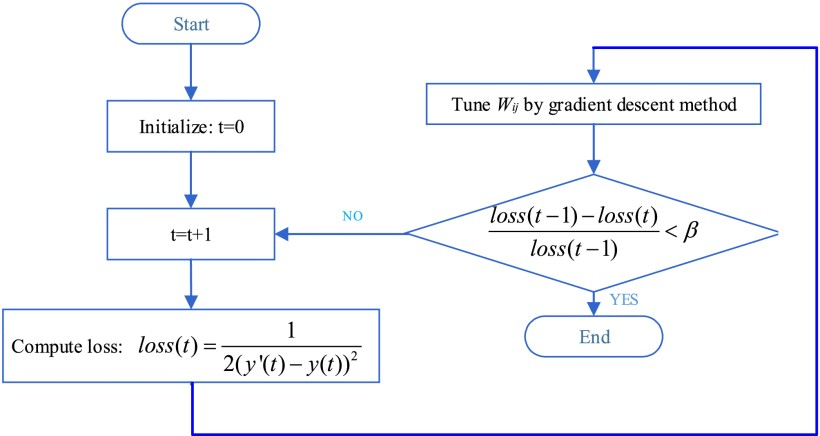
\includegraphics[width=0.8\textwidth]{baek4-2880511-large.jpg}
    \caption{Back-propagated fine-tuning process. \cite{baek2019}}
    \label{fig:example}
\end{figure}

% Add other chapters as needed
\chapter{Title of first paper}
This chapter has a table.


\begin{table}[ht]
    \centering
    \begin{tabular}{p{8cm}c}
        \toprule
    \textbf{Institution} & \textbf{Founding Date} \\ \midrule
    University of Virginia School of Data Science & 2019 \\ 
    Indiana University Luddy School of Informatics, Computing, and Engineering & 2015 \\ 
    University of California, Berkeley Division of Data Sciences & 2017 \\ 
    NYU Center for Data Science & 2013 \\ 
    University of Rochester Goergen Institute for Data Science & 2015 \\ \bottomrule
    \end{tabular}
    \caption{US Schools of Data Science and Their Founding Dates}
    \end{table}
    

\chapter{Title of second paper}
By placing the text of each chapter in its own file, you can use the file for the dissertation and for individual publications.  The formatting will automatically change depending on which document is being rendered.

\begin{figure}[h]
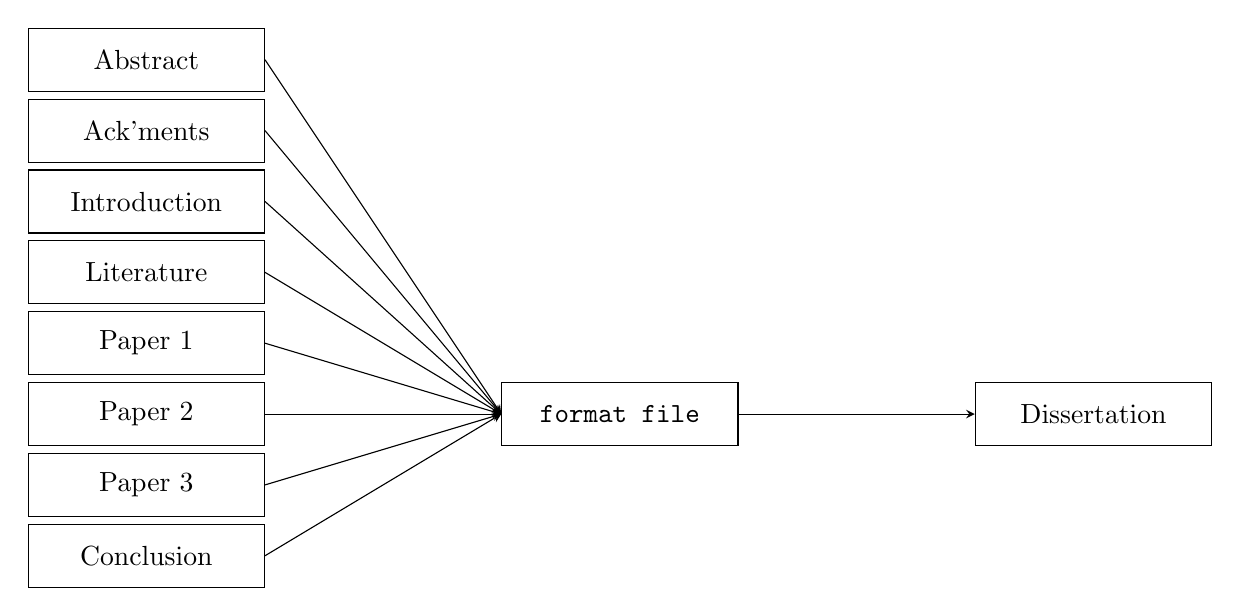
\begin{tikzpicture}[node distance=.9cm, every node/.style={draw, rectangle, minimum height=.8cm, minimum width=3cm}, >=stealth]

    % Left column nodes
    \node (abstract) {Abstract};
    \node (acknowledgements) [below of=abstract] {Ack'ments};
    \node (introduction) [below of=acknowledgements] {Introduction};
    \node (literature) [below of=introduction] {Literature};
    \node (paper1) [below of=literature] {Paper 1};
    \node (paper2) [below of=paper1] {Paper 2};
    \node (paper3) [below of=paper2] {Paper 3};
    \node (conclusion) [below of=paper3] {Conclusion};
    
    % Right column node
    \node (doc) [right=3cm of paper2] {\tt format file};
    \node (pdf) [right=3cm of doc] {Dissertation};
    
    % Arrows from each left box to the right box
    \draw[->] (abstract.east) -- (doc.west);
    \draw[->] (acknowledgements.east) -- (doc.west);
    \draw[->] (introduction.east) -- (doc.west);
    \draw[->] (literature.east) -- (doc.west);
    \draw[->] (paper1.east) -- (doc.west);
    \draw[->] (paper2.east) -- (doc.west);
    \draw[->] (paper3.east) -- (doc.west);
    \draw[->] (conclusion.east) -- (doc.west);
    \draw[->] (doc.east) -- (pdf.west);
    
\end{tikzpicture}

\rule{0em}{2em}


\begin{tikzpicture}[node distance=1.2cm, every node/.style={draw, rectangle, minimum height=.8cm, minimum width=3cm}, >=stealth]

    % Left column nodes
    \node (paper1) {Paper 1};
    
    % Right column node
    \node (doc) [right=3cm of paper1] {\tt format file};
    \node (pdf) [right=3cm of doc] {Journal article};

        % Arrows from each left box to the right box
    \draw[->] (paper1.east) -- (doc.west);
    \draw[->] (doc.east) -- (pdf.west);
    
\end{tikzpicture}
\caption{Why use {\tt input} when rendering your dissertation}
\end{figure}

\chapter{Title of third paper}

\chapter{Conclusion}

% Bibliography
\addcontentsline{toc}{chapter}{References}
\bibliographystyle{plain} 
\bibliography{references}

% Code and supplementary information
\chapter*{Code and supplementary files}  % Format like a chapter heading
\addcontentsline{toc}{chapter}{Code and supplementary files}  % Add it to the TOC
Code scripts and supplementary files for this dissertation are available at the following locations.

\begin{center}
\begin{tabular}{ll} \toprule
Files & Location \\ \midrule
Paper 1 & \href{https://www.github.com/username/reponame1}{github.com/username/reponame1} \\
Paper 2 & \href{https://www.github.com/username/reponame2}{github.com/username/reponame2} \\
Paper 2 & \href{https://www.github.com/username/reponame3}{github.com/username/reponame3} \\ \bottomrule
\end{tabular}
\end{center}

\newpage
% A unique databurst for each dissertation
\thispagestyle{empty}
\begin{tikzpicture}[overlay, remember picture, shift={(current page.center)}]
    % Define the radius of the large circle
    \def\Radius{.5} % radius for 1 inch diameter circle
    % Number of small circles
    \def\NumCircles{56}
    % Radius of small circles
    \def\SmallCircleRadius{0.05}
    \def\NumRows{24}
    \def\ColSkip{8}

    % Draw the large circle (optional, for reference)
    %\draw (0,0) circle (\Radius);

    % Calculate angle step
    \pgfmathsetmacro\AngleStep{360/\NumCircles}

    % Draw small circles along the path
\foreach \j in {1,...,\NumRows}
{
    \foreach \i in {1,...,\NumCircles}
    {
        \pgfmathsetmacro{\tp}{int(random(1,\NumRows)+1>=\j)}
        \ifnum\tp=0 \relax
          \else  
            \pgfmathsetmacro{\tp}{random(1,100)/100}
          \fi
        \pgfmathparse{int(Mod(\i,\ColSkip))}
        \ifnum\pgfmathresult=0 \relax
            \else
                \pgfmathsetmacro\Angle{\AngleStep*\i}
                \draw[gold, fill=gold, opacity=\tp] (\Angle:\Radius+\j*3*\SmallCircleRadius) circle (\SmallCircleRadius);
            \fi
    }
}
\end{tikzpicture}

% End of document
\end{document}
